\documentclass[a4paper, oneside, 10pt]{article}
\usepackage[utf8]{inputenc}
\usepackage[spanish]{babel}
\usepackage[T1]{fontenc}
\usepackage{graphicx}
\usepackage{longtable}
\usepackage{hyperref}
\hypersetup{
	colorlinks=true,
	citecolor=black,
	linkcolor=blue,
	filecolor=blue,      
	urlcolor=blue}
\usepackage[small]{caption}
\usepackage[figuresright]{rotating}
% Añade al índice los entornos subsubsection
\setcounter{tocdepth}{3}
\setcounter{secnumdepth}{3}
% Entornos multicolumna
\usepackage{multicol}
% Entornos de lista
\usepackage{enumitem}
% Entornos float (imagenes y demás)
\usepackage{floatrow}	% Permite poner a un lado los pies de imagen
\usepackage{subcaption}
% Entornos matemáticos y elementos matemáticos
\usepackage{amsmath}
\usepackage{amsfonts}
\usepackage{amssymb}
% Letaras y caracteres especiales (por problemas usando €)
\usepackage{marvosym}
\DeclareUnicodeCharacter{20AC}{\EUR{}}
% Entornos de tabla modificados
\usepackage{multirow}
\usepackage{array}
\newcolumntype{M}[1]{>{\raggedright\let\newline\\\arraybackslash\hspace{0pt}}m{#1}}
\newcolumntype{N}[1]{>{\centering\let\newline\\\arraybackslash\hspace{0pt}}m{#1}}
\newcolumntype{P}[1]{>{\raggedleft\let\newline\\\arraybackslash\hspace{0pt}}m{#1}}
\usepackage{tabulary}
\usepackage{longtable}
% Entorno que permiten generar colores
\usepackage[table, dvipsnames]{xcolor}
%%%% Gris muy claro
\definecolor{hiperlightgray}{gray}{0.85}
% Entornos para añadir algoritmos y fragmentos de código
\usepackage[ruled,vlined]{algorithm2e}
\usepackage{listings}
\lstset{
    backgroundcolor=\color{hiperlightgray},   % Indica el color de fondo; necesita que se añada \usepackage{color} o \usepackage{xcolor}
    basicstyle=\scriptsize,
    showstringspaces=false,
    formfeed=newpage,
    tabsize=4,
    commentstyle=\itshape,
    morekeywords={models, lambda, forms}
}

% set margins for double-sided printing
\usepackage[left=1.2cm, right=1.2cm, top=1.4cm, bottom=1.4cm, bindingoffset=1.2cm, head=15pt]{geometry} 
\usepackage{setspace}
\onehalfspacing
% set headers
\usepackage{fancyhdr}
\pagestyle{fancy}
\fancyhead{}
\fancyfoot{}
\fancyhead[L,RO]{\textsl{\leftmark}}
\fancyhead[R,LO]{\thesisauthor}
\fancyfoot[C]{\thepage}
\renewcommand{\headrulewidth}{0.4pt}
\renewcommand{\footrulewidth}{0pt}

% set APA citation style
\usepackage{apacite}
\usepackage[numbib,notlof,notlot,nottoc]{tocbibind}
\pagenumbering{gobble}

%%%%%%%%%%%%%%%%%%%%%%%%%%%%%%%%%%%%%%%%%%%%%%%%%%%%%%%%%%%%%
%THESIS Parameters 
%%%%%%%%%%%%%%%%%%%%%%%%%%%%%%%%%%%%%%%%%%%%%%%%%%%%%%%%%%%%%

\title{}

\newcommand{\thesisdate}{\today}
\newcommand{\thesisauthor}{Alejandro Cebrián del Valle} %input name
\newcommand{\studentID}{70907} %input student ID
\newcommand{\thesistype}{Recopilatorio} % Set either to Bachelor or Master
\newcommand{\proyecto}{Fundación para la Investigación Biomédica Hospital Clínico San Carlos}

%%%%%%%%%%%%%%%%%%%%%%%%%%%%%%%%%%%%%%%%%%%%%%%%%%%%%%%%%%%%%
%DOCUMENT
%%%%%%%%%%%%%%%%%%%%%%%%%%%%%%%%%%%%%%%%%%%%%%%%%%%%%%%%%%%%%
\begin{document}
	%%%%%%%%%%%%%%%%%%%%%%%%%%%%%%%%%%%%%%%%%%%%%%%%%%%%%%%%%%%%%
	%TITLE PAGE (Pre-defined, just change parameters above)
	%%%%%%%%%%%%%%%%%%%%%%%%%%%%%%%%%%%%%%%%%%%%%%%%%%%%%%%%%%%%%
	%%%%%%%%%%%%%%%%%%%%%%%%%%%%%%%%%%%%%%%%%%%%%%%%%%%%%%%%%%%%%
%TITLE PAGE
%%%%%%%%%%%%%%%%%%%%%%%%%%%%%%%%%%%%%%%%%%%%%%%%%%%%%%%%%%%%%
\makeatletter
\begin{titlepage}
	\begin{center}
		\vspace*{1cm}
		
		\Large
		\textbf{\@title}
		
		\vspace{1.5cm}
		
		\thesistype{}
		
		\vspace{1cm}
		
		%\begin{figure}[htbp]
		%	\centering
		%	\includegraphics[width=.7\linewidth]{./figuras/Escudo.png}
		%\end{figure}
		
		\vspace{1cm}
		
		\Large
		\textbf{Autor}: \thesisauthor{}\\ (N empleado: \studentID{})\\
		\Large
		\textbf{} \proyecto{}\\
		%\large
		%\textbf{Coautor}: \cosupervisor{}
		
		\vspace{2cm}
		\large
		%Department of Information Systems for Sustainable Society\\
		%Faculty of Management, Economics and Social Sciences\\
		%University of Cologne\\
		
		\vspace{1cm}
		\@date
		
	\end{center}
\end{titlepage}
\makeatother
	%%%%%%%%%%%%%%%%%%%%%%%%%%%%%%%%%%%%%%%%%%%%%%%%%%%%%%%%%%%%%
	%TOC,TOF,TOT
	%%%%%%%%%%%%%%%%%%%%%%%%%%%%%%%%%%%%%%%%%%%%%%%%%%%%%%%%%%%%%
	\clearpage
	\pagenumbering{Roman}
	\begingroup
		\hypersetup{hidelinks}
		\tableofcontents
		\section*{Resumen}      
			
		%\clearpage
		\listoffigures
		\listoftables
	\endgroup
	\clearpage
	\pagenumbering{arabic}
	%%%%%%%%%%%%%%%%%%%%%%%%%%%%%%%%%%%%%%%%%%%%%%%%%%%%%%%%%%%%%
	%MAIN PART
	%%%%%%%%%%%%%%%%%%%%%%%%%%%%%%%%%%%%%%%%%%%%%%%%%%%%%%%%%%%%%
	%\part{Introducción}
	% SEC I - Aula
	\section{Soporte Vital Inmediato}
\subsection{Estaciones y cronograma}
Las estaciones y el cronograma se hacen de acuerdo a lo hecho en el curso de SVI de noviembre de 2022. 

% Please add the following required packages to your document preamble:
% \usepackage{multirow}
% \usepackage[table,xcdraw]{xcolor}
% If you use beamer only pass "xcolor=table" option, i.e. \documentclass[xcolor=table]{beamer}
\begin{table}[hptb]
    \centering
    \begin{tabular}{ccccc}
    \rowcolor[HTML]{333333} 
    {\color[HTML]{FFFFFF} Día} & {\color[HTML]{FFFFFF} Duración} & {\color[HTML]{FFFFFF} Grupo A} & {\color[HTML]{FFFFFF} Grupo B} & {\color[HTML]{FFFFFF} Grupo C} \\
     & 1 H & \multicolumn{3}{c}{Explicación Teórica} \\
     & \cellcolor[HTML]{D9D9D9}45 min & \multicolumn{3}{c}{\cellcolor[HTML]{D9D9D9}RCP básica} \\
     & 45 min & \multicolumn{3}{c}{Aproximación ABCDE} \\
     & \cellcolor[HTML]{D9D9D9}15/30 min & \multicolumn{3}{c}{\cellcolor[HTML]{D9D9D9}Descanso} \\
     & 45 min & Vía aérea & Acceso Vascular, fármacos & Monitorización y arritmias \\
     & \cellcolor[HTML]{D9D9D9}45 min & \cellcolor[HTML]{D9D9D9}Monitorización y arritmias & \cellcolor[HTML]{D9D9D9}Vía aérea & \cellcolor[HTML]{D9D9D9}Acceso Vascular,  fármacos \\
    \multirow{-7}{*}{Día I} & 45 min & Acceso Vascular, fármacos & Monitorización y arritmias & Vía aérea \\ \hline
    \rowcolor[HTML]{D9D9D9} 
    \cellcolor[HTML]{D9D9D9} & 1 H & \multicolumn{3}{c}{\cellcolor[HTML]{D9D9D9}Escenarios de SVI y desfibrilación} \\
    \cellcolor[HTML]{D9D9D9} & 30 min & \multicolumn{3}{c}{Demostración SVI integrado} \\
    \rowcolor[HTML]{D9D9D9} 
    \cellcolor[HTML]{D9D9D9} & 1 H & \multicolumn{3}{c}{\cellcolor[HTML]{D9D9D9}Escenario Integrado SVI} \\
    \cellcolor[HTML]{D9D9D9} & 20 min & \multicolumn{3}{c}{Descanso} \\
    \rowcolor[HTML]{D9D9D9} 
    \multirow{-5}{*}{\cellcolor[HTML]{D9D9D9}Día II} & $\mathbb{N}$ min & \multicolumn{3}{c}{\cellcolor[HTML]{D9D9D9}Evaluación} \\ \hline
    \end{tabular}
    \caption{Estaciones propuestas para SVA junto con su duración}
    \label{tab:Brusilov:SVI:Estaciones}
\end{table}

% Please add the following required packages to your document preamble:
% \usepackage[table,xcdraw]{xcolor}
% If you use beamer only pass "xcolor=table" option, i.e. \documentclass[xcolor=table]{beamer}
\begin{table}[hptb]
    \centering
    \begin{tabular}{N{0.25\textwidth}N{0.2\textwidth}M{0.45\textwidth}}
        \rowcolor[HTML]{333333} 
        {\color[HTML]{FFFFFF} Estación} & {\color[HTML]{FFFFFF} Sala propuesta} & {\color[HTML]{FFFFFF} Equipamiento} \\
        Explicación teórica & Aula 2 (Debriefing I) & Ordenador, Pantalla, Sillas \\
        \rowcolor[HTML]{D9D9D9} 
        RCP Básica & Simulación 1, Simulación 2, Simulación 3 & Busto RCP, DEA Laerdal \\
        Aproximación ABCDE & Simulación 1, Simulación 2, Simulación 3 & Sillas \\
        \rowcolor[HTML]{D9D9D9} 
        Vía Aérea, Oxigenoterapia y Ventilación & Simulación 1 & Gafas Nasales, Mascarillas faciales (con reservorio, efecto Venturi), Cánula de Guedel, Mascarilla laríngea (clásica, iGel), Fastrach (Fastrach, tubo de Brian, intercambiador), Tubo endotraqueal, Laringoscopio, Froba, Fiador, Kit cricotirotomía, Airtraq, Sonda Yankauer, Tubuladuras para respirador, Ambú, Busto para intubación \\
        Acceso Vascular, líquidos y fármacos & Simulación 2 & Abbocat de distintos tamaños, pistola intraósea, aguja para intraósea, muslo de pollo y huevos, brazo para venopunción \\
        \rowcolor[HTML]{D9D9D9} 
        Monitorización y Arritmias & Simulación 3 & Desfibrilador, maniquí simulador arritmias, DEA \\
        Escenarios SVI y desfibrilación & Simulación 1, Simulación 2, Simulación 3 & Sillas \\
        \rowcolor[HTML]{D9D9D9} 
        Escenarios Integrados SVI/Demostración SVI & Simulación 3 y Aula 2 (Debriefing I) & Abbocat de distintos tamaños, ampollas medicación Mock, Sueros y sistemas de suero, Gafas Nasales, Mascarillas faciales (con reservorio, efecto Venturi), Cánula de Guedel, Mascarilla laríngea (clásica, iGel), Fastrach (Fastrach, tubo de Brian, intercambiador), Tubo endotraqueal, Laringoscopio, Froba, Fiador, Tubuladuras para respirador, Aula Debriefing I (Sistema Intuity, Ordenador, Pantalla) \\ \hline
    \end{tabular}
    \caption{Salas y material propuesto para cada estación descrita}
    \label{tab:Brusilov:SVI:SalasEstaciones}
\end{table}

Así, el listado de materiales queda (según lo pedido en la información dada):
\begin{itemize}[topsep=0pt, partopsep=0pt,itemsep=0pt,parsep=0pt]
    \item \textbf{Medicación y Material de vía venosa}:
    \begin{itemize}[topsep=0pt, partopsep=0pt,itemsep=0pt,parsep=0pt]
        \item 30 Apósitos.
        \item Catéter Abbocat (30 del 24G, 30 del 22G, 30 del 20G, 2 del 18G, 2 del 16G, 2 del 14G).
        \item 2 Compresor.
        \item Bolsa de Sangre y de Plasma para transfusiones.
        \item Material de intraósea (pistola de intraósea, agujas para intraósea).
        \item Ampollas de Medicación Mock (reetiquetar suero fisiológico de uso tópico):
        \vspace{-12.5pt}
        \begin{multicols}{2}
            \begin{itemize}[topsep=0pt, partopsep=0pt,itemsep=0pt,parsep=0pt]
                \item Ácido tranexámico 500 mg (100 mg/mL).
                \item Adrenalina 1 mg/mL.
                \item Alteplasa 100 mg (20 mg/mL).
                \item Amiodarona 150 mg (50 mg/mL).
                \item Atropina 1 mg/mL.
                \item Bicarbonato sódico 1 M (8.5 mg/mL).
                \item Bicarbonato sódico 1.6 M (14 mg/mL).
                \item Cloruro Sódico 20 \% (200 mg/mL).
                \item Cloruro Cálcico 100 mg (100 mg/mL).
                \item Cloruro Potásico 20 mEq (2mEq/mL).
                \item Digoxina 0.5 mg (0.25 mg/mL).
                \item Dopamina 200 mg (40 mg/mL).
                \item Etomidato 20 mg (2 mg/mL).
                \item Fentalino 0.5 mg (0,15 mg/mL).
                \item Fibrinógeno 1 g (20 mg/mL).
                \item Hidrocortisona 100 mg (20 mg/mL).
                \item Hidroxicobalamina 100 mg (5000 $\mu$g/mL).
                \item Labetalol 100 mg (5 mg/mL).
                \item Lidocaína 2 \% 200 mg (20 mg/mL).
                \item Matamizol magnésico 2g (0.04 mg/mL).
                \item Midozalam 15 mg (5mg/mL).
                \item Morfina 10 mg/mL
                \item Nitroglicerina 50 mg (5 mg/mL).
                \item Noradrenalina 10 mg (2 mg/mL).
                \item Propofol 200 mg (10 mg/mL).
                \item Rocuronio 50 mg (10 mg/mL)
                \item Sulfato magnésico 1,5 mg (150 mg/mL).
                \item Urapidilo 50 mg (5 mg/mL).
            \end{itemize}
        \end{multicols}
    \end{itemize}
    \item \textbf{Material de vía aérea}:
    \begin{itemize}[topsep=0pt, partopsep=0pt,itemsep=0pt,parsep=0pt]
        \item Busto de intubación Laerdal.
        \item 2 Gafas Nasales.
        \item 4 Mascarillas faciales (2 efecto Venturi, 2 con reservorio).
        \item Canulas de Guedel (2 de cada calibre).
        \item 2 Mascarillas laríngeas clásicas Calibre 3.
        \item Mascarillas laríngeas iGel (2 de cada calibre).
        \item 2 Mascarillas Fastrach (calibre 3), junto con tubo de Brian e intercambiador.
        \item Tubo orotraqueal (2 de cada calibre: 6, 6.5, 7, 7.5, 8).
        \item 2 Laringoscopios.
        \item 2 Airtraq
        \item 2 Botes de lubricante para intubación.
        \item 2 Sonda Yankauer, junto con sistema de vacio.
        \item 2 Pinzas de Magill.
        \item Kit de cricotirotomía.
        \item 2 Tubuladuras de respirador.
    \end{itemize}
    \item \textbf{Otros}:
    \begin{itemize}[topsep=0pt, partopsep=0pt,itemsep=0pt,parsep=0pt]
        \item Drenaje con sangre.
        \item Pleurevac.
        \item Sábana Pélvica.
        \item Collarín.
        \item Tubo de tórax.
        \item Vendas.
        \item Catéter Central de Inserción Periférica (PICC).
    \end{itemize}
\end{itemize}
\subsection{Casos Codificados}
\subsubsection{Caso A - Asistolia por Shock hipovolémico}
\paragraph{Escenario} UCI
\paragraph{Paciente} Varón de 60 años, hipertenso y obeso. Intervenido resección sigma hace 12 horas. El paciente presenta una hipotensión brusca (70/40 mmHg), taquicardia sinusal (110 lpm), sudoración y malestar general tras administrar un nolotil intravenoso. El paciente lleva un drenaje abdominal con débito hemático. Enfermería avisa al personal médico de guardia.
\paragraph{Caso} Enfermería avisa al personal médico de guardia. Paciente relata que le han operado, tras 100 segundos, pierde conocimiento (deja de hablar) y deja de notarse el pulso. Presenta una Actividad eléctrica sin pulso (shock hipovolémico).

Se espera que el alumnado realice el protocolo de RCP no desfibrilable:
\begin{enumerate}[topsep=0pt, partopsep=0pt,itemsep=0pt,parsep=0pt]
    \item Colocación de tablero de RCP.
    \item Inicio de compresiones y asistencia de vía aérea con Ambú (30:2).
    \item Canalización de vía venosa, junto con administración de medicación (adrenalina cada 3 minutos).
    \item Si el alumnado no progresa (sólo hace compresiones), recordar las posibles causas de parada (<<4H y 4T>>).
\end{enumerate}

\paragraph{Pruebas complementarias}
\begin{itemize}[topsep=0pt, partopsep=0pt,itemsep=0pt,parsep=0pt]
    \item\textbf{Gasometría de ingreso}: pH 7,40; pCO$_2$ 45; pO$_2$ 20; EB -3; lact 8; Hb 10; HCO$_3^-$ 25.
    \item \textbf{Gasometría preparada}: pH 7,10; pCO$_2$ 50; pO$_2$ 20; EB -15; lact 8; Hb 7; HCO$_3^-$ 16.
    \item \textbf{Gasometría en parada}: pH 7,00; pCO$_2$ 50; pO$_2$ 20; EB -20; lact 8; Hb 5; HCO$_3^-$ 12.
    \item \textbf{Ecografía}: %%TODO Enlace a Ecografía
\end{itemize}

\begin{figure}[hptb]
    \centering
	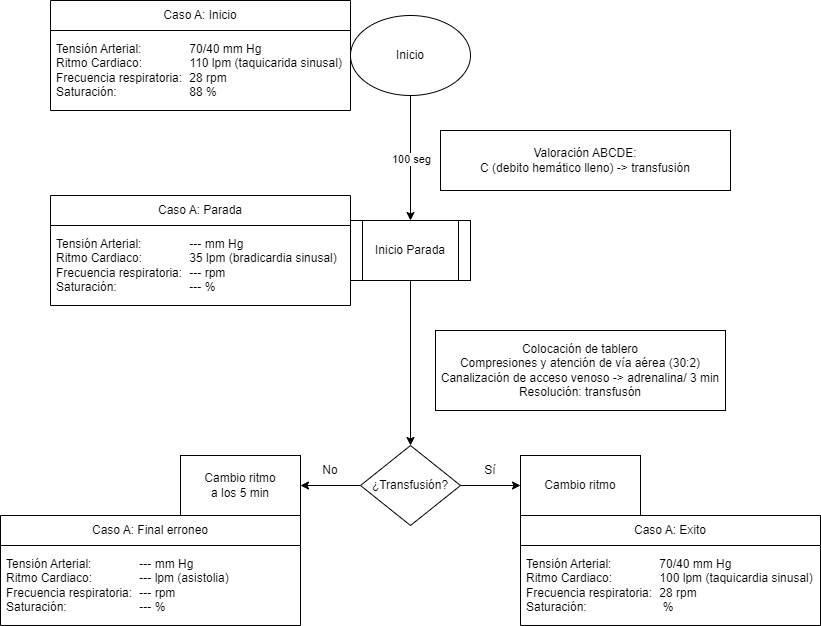
\includegraphics[width=\linewidth]{./imagenes/ACV-AdSC-CasosUCI_CasoA.png}
	\caption{\label{fig:Brusilov:SVI:CasoA}Flujograma y resolución del Caso A.}
\end{figure}
\subsubsection{Caso B - Taquicardia Ventricular con Pulso}
\paragraph{Escenario} Urgencias
\paragraph{Paciente} Mujer de 65 años acude a urgencias con 
\paragraph{Caso} Enfermería avisa al personal médico de guardia. Paciente relata que le han operado, tras 100 segundos, pierde conocimiento (deja de hablar) y deja de notarse el pulso. Presenta una Actividad eléctrica sin pulso (shock hipovolémico).

Se espera que el alumnado realice el protocolo de RCP no desfibrilable:
\begin{enumerate}[topsep=0pt, partopsep=0pt,itemsep=0pt,parsep=0pt]
    \item Colocación de tablero de RCP.
    \item Inicio de compresiones y asistencia de vía aérea con Ambú (30:2).
    \item Canalización de vía venosa, junto con administración de medicación (adrenalina cada 3 minutos).
    \item Si el alumnado no progresa (sólo hace compresiones), recordar las posibles causas de parada (<<4H y 4T>>).
\end{enumerate}

\paragraph{Pruebas complementarias}
\begin{itemize}[topsep=0pt, partopsep=0pt,itemsep=0pt,parsep=0pt]
    \item \textbf{Gasometría preparada}: pH 7,10; pCO$_2$ 50; pO$_2$ 20; EB -15; lact 8; Hb 7; HCO$_3^-$ 16.
    \item \textbf{Gasometría en parada}: pH 7,00; pCO$_2$ 50; pO$_2$ 20; EB -20; lact 8; Hb 5; HCO$_3^-$ 12.
    \item \textbf{Electrocardiograma previo}: %%TODO Enlace a ECG
    \item \textbf
\end{itemize}

\begin{figure}[hptb]
    \centering
	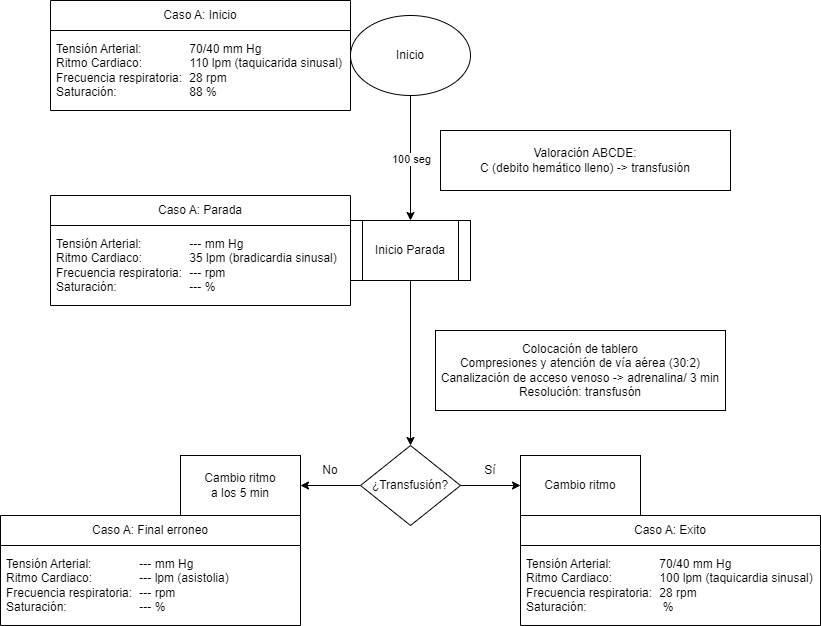
\includegraphics[width=\linewidth]{./imagenes/ACV-AdSC-CasosUCI_CasoA.png}
	\caption{\label{fig:Brusilov:SVI:CasoA}Flujograma y resolución del Caso A.}
\end{figure}



	%%%%%%%%%%%%%%%%%%%%%%%%%%%%%%%%%%%%%%%%%%%%%%%%%%%%%%%%%%%%%
	%APPENDICES
	%%%%%%%%%%%%%%%%%%%%%%%%%%%%%%%%%%%%%%%%%%%%%%%%%%%%%%%%%%%%%
	%\part*{Apendices}
	%\appendix
	%\clearpage
	%\renewcommand*{\thesection}{\Alph{section}}\textbf{}
	%\input{./secciones/ACV-GlosarioBiomedicoGRU}
	%%%%%%%%%%%%%%%%%%%%%%%%%%%%%%%%%%%%%%%%%%%%%%%%%%%%%%%%%%%%%
	%BIBLIOGRAPHY
	%%%%%%%%%%%%%%%%%%%%%%%%%%%%%%%%%%%%%%%%%%%%%%%%%%%%%%%%%%%%%
	%\part{Adendas}
	%\renewcommand*{\thesection}{}\textbf{}
	\bibliographystyle{apacite}
	%\bibliography{secciones/Bibliography}
\end{document}
